\documentclass{seminar}

% Use latex filename for dvi output and pdflatex file for pdf output.

\usepackage[dvips]{graphicx}

% \usepackage[pdftex]{graphicx} does not seem to be needed.

\DeclareGraphicsExtensions{.eps,.ps,.pdf,.jpg}

\usepackage{alltt} % 
\usepackage{fancybox} % For making Oval borders.
\usepackage{amssymb}  % For, for example, \mathbb, \big, and \mapsto
\usepackage{url} % For email addresses, hypertext links, ...
\usepackage{color} % For color.
\usepackage{hyperref} % For hyper reference but *essential* for seminar.
\usepackage{multicol}

% Options for hyperref.

\hypersetup{pdfpagemode=none,pdfstartview=FitH} % For the initial view.
\hypersetup{colorlinks=true}
\hypersetup{hypertexnames=false} % Eliminates message: pdfTeX warning (ext4)
\hypersetup{urlcolor=red}

% Basic definitions.

\renewcommand{\printlandscape}{\special{landscape}}    % Works with dvips.
\newcommand{\R}{\mbox{${\mathbb R}$}}
\newcommand{\C}{\mbox{${\mathbb C}$}}
\newcommand{\grad}{\nabla}
\setlength{\jot}{0.0pt}
\newcommand{\half}{{\textstyle{\frac{1}{2}}}}
\newcommand{\third}{{\textstyle{\frac{1}{3}}}}
\newcommand{\codes}[1]{{\textsf{\footnotesize #1}}}

% Calligraphic letter abbreviations.

\newcommand{\cA} {\mbox{$\cal A$}}
\newcommand{\cP} {\mbox{$\cal P$}}
\newcommand{\cS} {\mbox{$\cal S$}}
\newcommand{\cT} {\mbox{$\cal T$}}

% Color symbols.

\newcommand{\redball}{\textcolor{red}{$\bullet$}}
\newcommand{\reddash}{\textcolor{red}{$--$}}
\newcommand{\reddiamond}{\textcolor{red}{$\diamond$}}
\newcommand{\redcircle}{\textcolor{red}{$\circ$}}
\newcommand{\redstar}{\textcolor{red}{$\star$}}
\newcommand{\redrightarrow}{\textcolor{red}{$\Rightarrow$}}

\newcommand{\redstripe}{\textcolor{red}{\hrule height 2.0pt\hfil}
             \vspace{-1.8pt}
             \textcolor{red}{\hrule height 1.0pt\hfil}
}

\newcommand{\heading}[1]{%
   \centerline{\textcolor{blue}{\textbf{#1}}}%
    \redstripe%
    \bigskip
}

% Script letters.

\newcommand{\cD} {\mbox{$\cal D$}}

\newpagestyle{MH}
{}
{\hfil 
\includegraphics[scale=0.15]{../images/lans-c}}

\pagestyle{MH}
% \pagestyle{empty}

\slideframe{Oval}
\slideframe{none}

% \twoup

\begin{document}

\begin{slide}

\begin{center}
{\bf
Workshop on the ACTS Toolkit \\
October 10--13, 2001 \\
National Energy Research Scientific Computing Center
}
\end{center}

\redstripe

\begin{center}
{\bf
\textcolor{blue}{TAO -- Toolkit for Advanced Optimization}
}

\redstripe

\medskip

\centerline{\textbf{Steve Benson, Lois Curfman McInnes, and Jorge J. Mor\'e}}

\end{center}

% \medskip

\parbox[b]{3in}{\url{http://www.mcs.anl.gov/tao} \bigskip \\
\small  Mathematics and Computer Science Division \\ 
Argonne National Laboratory} 
\includegraphics[scale=0.5]{../images//argonne}

\end{slide}

\begin{slide}

\heading{Outline}

\begin{list}{\reddiamond}{}
\item
Optimization background
\item
TAO
\begin{list}{\redcircle}{}
\item
Algorithms
\item
Interface
\item
Usage
\end{list}
\end{list}

\vfill

\end{slide}

\begin{slide}

\heading{What is Nonlinearly Constrained Optimization?}

\[
\min \left \{ f(x): x_l \le x \le x_u , \ c_l \le c(x) \le c_u \right \}
\]

\medskip

\begin{list}{\reddiamond}{\setlength{\itemsep}{0pt}}
\item
Systems of nonlinear equations
\[
\min \left \{ \half \| r(x) \|^2 : x_l \le x \le x_u \right \} , \qquad
r : \R^n \mapsto \R^n
\]
\item
Nonlinear least squares
\[
\min \left \{ \half \| r(x) \|^2 : x_l \le x \le x_u \right \} , \qquad
r : \R^n \mapsto \R^m, \quad m \ge n
\]
\item
Bound-constrained optimization
\[
\min \left \{  f(x) : x_l \le x \le x_u \right \}
\]
\end{list}

\vfill

\end{slide}

%  \begin{slide}
%  
%  \heading{What is Nonlinearly Constrained Optimization?}
%  
%  \[
%  \min \left \{ f(x): x_l \le x \le x_u , \ c_l \le c(x) \le c_u \right \}
%  \]
%  
%  \medskip
%  
%  \begin{list}{\reddiamond}
%  {
%  % \setlength{\itemsep}{0pt}
%  }
%  \item
%  Unconstrained optimization
%  \[
%  \min \left \{  f(x) : x \in \R^n \right \}
%  \]
%  \item
%  Bound-constrained optimization
%  \[
%  \min \left \{  f(x) : x_l \le x \le x_u \right \}
%  \]
%  \item
%  Linear and quadratic programming
%  \[
%  \min \left \{ \half x^T Q x + c^T x : x_l \le x \le x_u , 
%  \ c_l \le Ax \le c_u \right \}
%  \]
%  \end{list}
%  
%  \vfill
%  
%  \end{slide}

\begin{slide}

\heading{The Ginzburg-Landau Model for Superconductivity}

Minimize the Gibbs free energy for a homogeneous superconductor with a vector
potential perpendicular to the superconductor.

{\small
\[
\int _ {\cD} \bigl \{ - | v (x) |^2 + \half | v (x) |^4  + 
\left \| \left [ \nabla - i A(x) \right ] v (x) \right \| ^2  +  \\
\kappa^2 \left \| ( \grad \times A ) (x) \right \| ^2 \bigr \} dx
\]
}

\medskip

\begin{center}
$ v : \R^2 \to \C$ is the order parameter

$A : \R^2 \to \R^2 $ is the vector potential
\end{center}

\vfill

\end{slide}

\begin{slide}

\heading{The Ginzburg-Landau Model for Superconductivity}

Unconstrained problem. Non-convex function. Hessian is singular.
Unique minimizer, but there is a saddle point.

\bigskip

\centerline {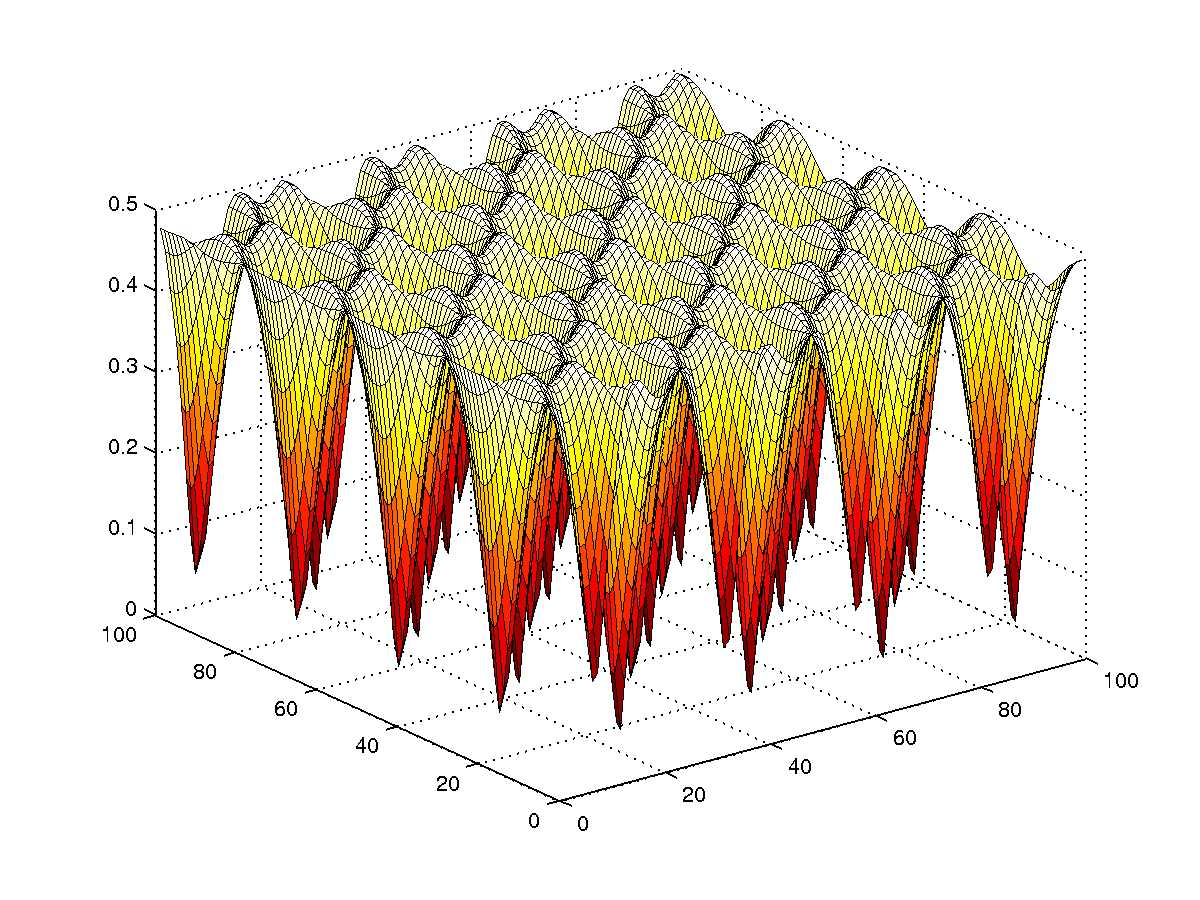
\includegraphics[height=1.5in]{../images/gl2_s}
             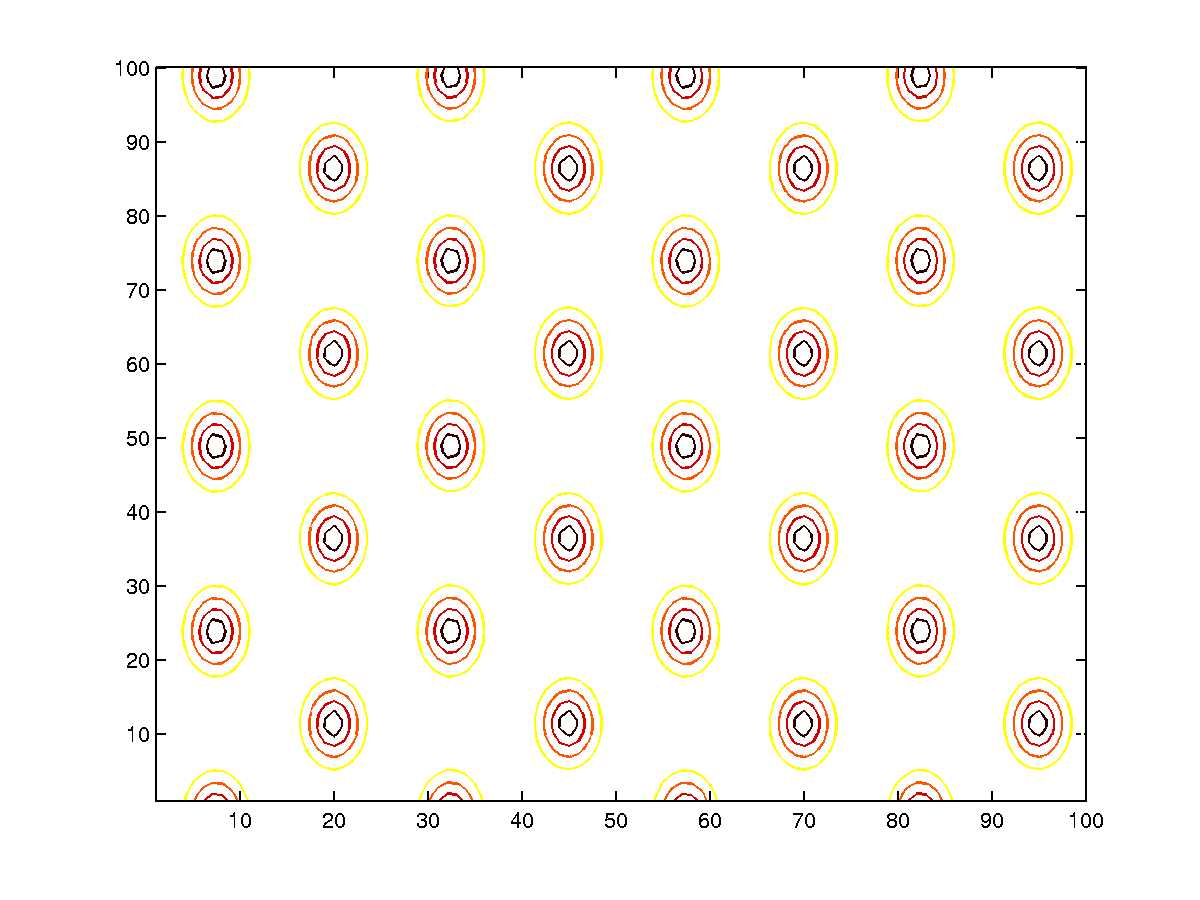
\includegraphics[height=1.5in]{../images/gl2_c}}

\end{slide}

\begin{slide}

\heading{Minimal Surface with Obstacles}

Determine the surface of minimal area and given boundary data
that lies above an obstacle.

\[
\min \left \{ f(v) : v \in K \right \}
\]

\[
f(v) = \int_{\cD} \sqrt{ 1 + \| \grad v(x) \|^2 } \; dx
\]

\[
K = \left \{ v \in H^1 : v(x) = v_D (x) , \ x \in \partial D, \ 
                v(x) \ge v_L (x) ,\  x \in \cD \right \}
\]

\vfill

\end{slide}

\begin{slide}

\heading{Minimal Surface with Obstacles}

Bound constrained problem. 
Number of active constraints depends on the height of the
obstacle. Almost all multipliers are zero. 

\bigskip

\centerline {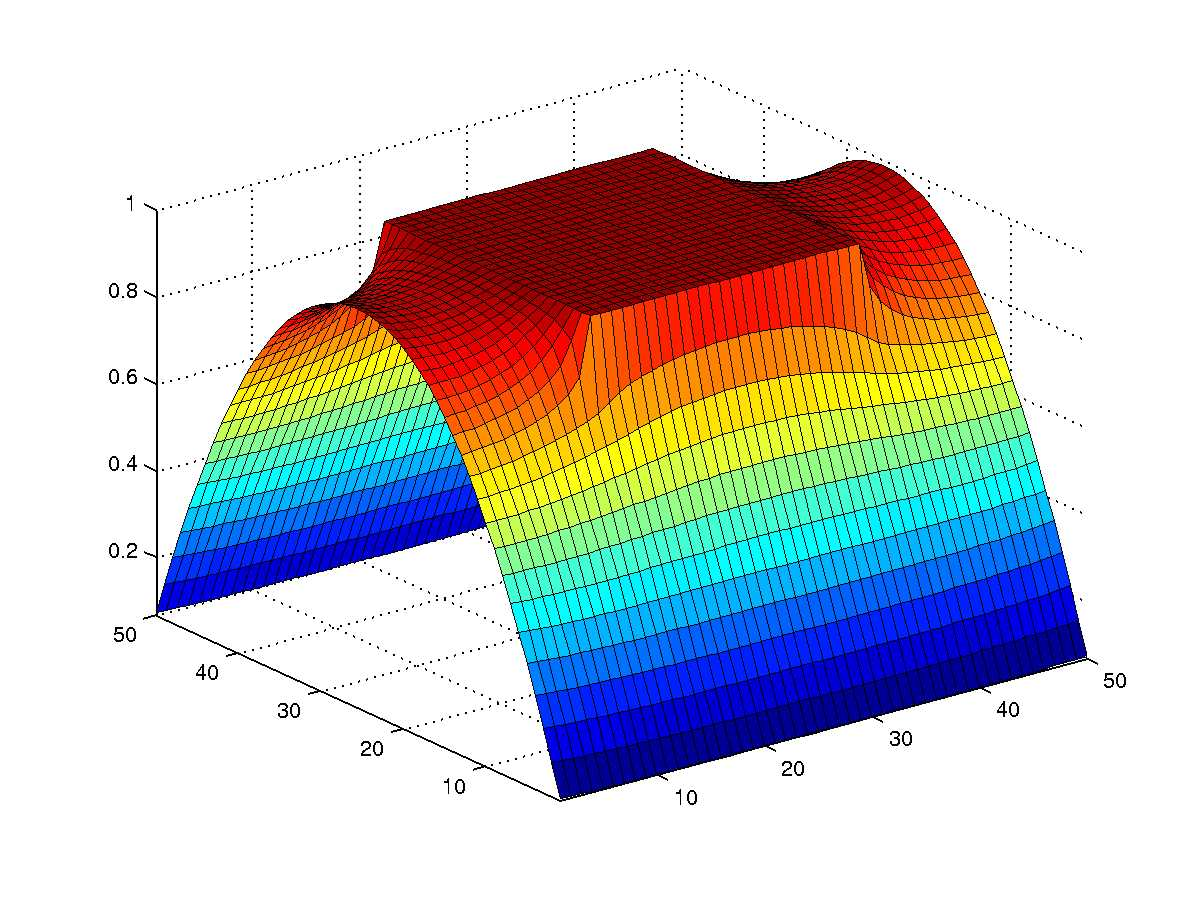
\includegraphics[height=1.5in]{../images/mso_s}
             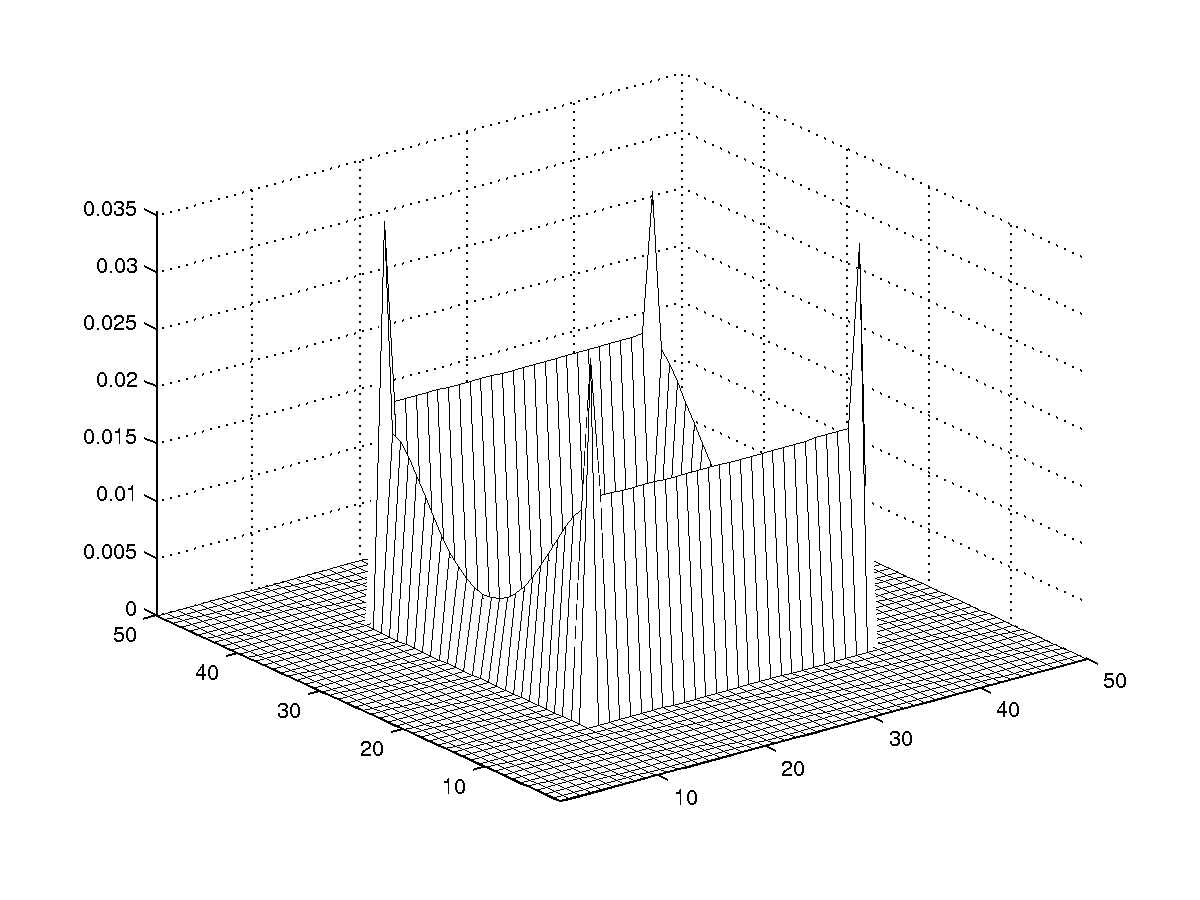
\includegraphics[height=1.5in]{../images/mso_e}}

\end{slide}



\begin{slide}

\heading{Isomerization of $ \alpha $-pinene}

Determine the reaction coefficients
in the thermal isometrization of $\alpha$-pinene from measurements by minimizing
\[
\sum _ {j=1}^8 \| y ( \tau_j ; \theta ) - z_j \| ^ 2 ,
\]
where $z_j$ are the measurements and
\begin{eqnarray*}
y_1'  & = & -(\theta_1 + \theta_2) y_1 \\
y_2'  & = & \theta_1 y_1 \\
y_3'  & = & \theta_2 y_1 - (\theta_3 + \theta_4 )y_3 + \theta_5 y_5 \\
y_4'  & = & \theta_3 y_3 \\
y_5'  & = & \theta_4 y_3 - \theta_5 y_5 \nonumber
\end{eqnarray*}

\vfill

\end{slide}

\begin{slide}

\heading{Isomerization of $\alpha$-pinene}

Only equality constraints. Typical parameter estimation problem. 

\bigskip

\centerline {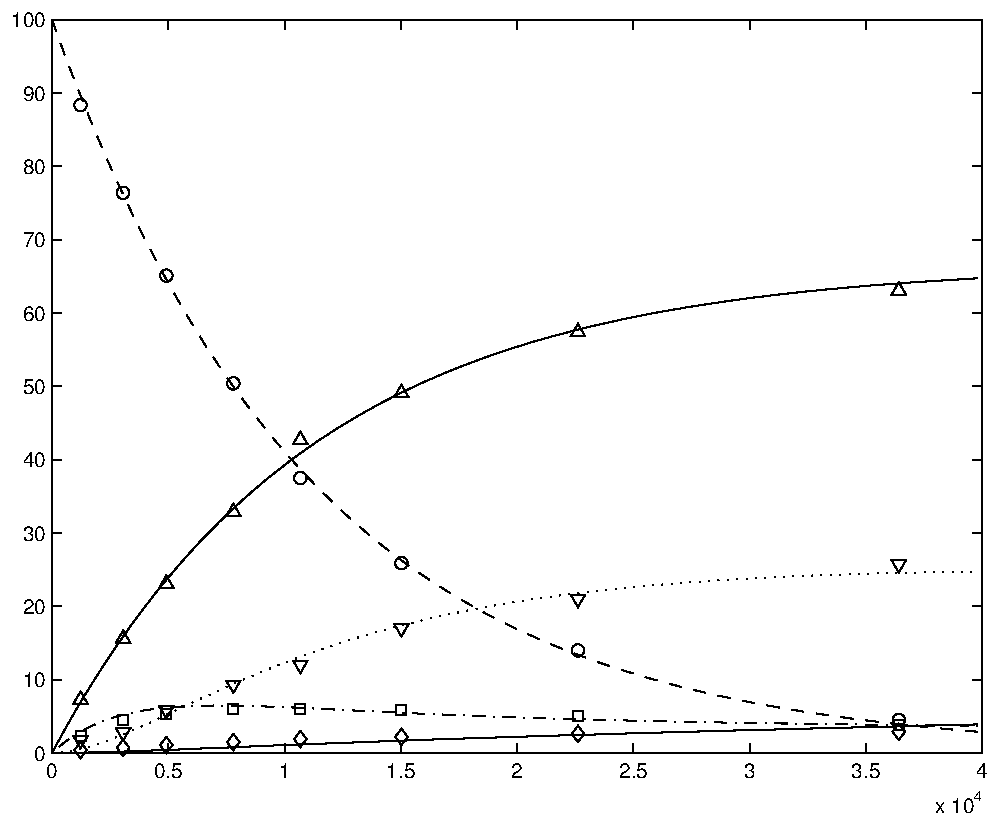
\includegraphics[height=1.8in]{../images/pinene}}

\vfill

\end{slide}

\begin{slide}

\heading{Optimization Toolkits}

State-of-the-art in optimization software:

\begin{list}{\reddiamond}{}
\item
Scattered support for parallel computations
\item
Little reuse of linear algebra software
\item
Minimal use of automatic differentiation software
\item
Few object-oriented optimization codes
\item
Nonlinear optimization problems with more than $ 10, 000 $
variables are considered large.
\end{list}

\vfill

\end{slide}

\begin{slide}

\heading{TAO}

The process of nature by which all things change
and which is to be followed for a life of harmony.

\bigskip

\begin{center}
\textcolor{red}{The Right Way}
\end{center}

\bigskip

Toolkit for advanced optimization

\begin{list}{\reddiamond}{}
\item
Object-oriented techniques
\item
Component-based interaction
\item
Leverage of existing parallel computing infrastructure
\item
Reuse of external toolkits
\end{list}

\vfill

\end{slide}

\begin{slide}

\heading{TAO Goals}

\begin{list}{\reddiamond}{}
\item
Portability
\item
Performance
\item
Scalable parallelism
\item
An interface independent of architecture
\end{list}

\vfill

\end{slide}


\begin{slide}

\heading{TAO Algorithms for Bound-Constrained Optimization}

\[
\min \left \{  f(x) : x_l \le x \le x_u \right \}
\]

\medskip

\begin{list}{\reddiamond}{}
\item
Conjugate gradient algorithms
\item
Limited-memory variable-metric algorithms
\item
Newton algorithms
\end{list}

You must supply the function $ f : \R^n \mapsto \R $ and the
gradient 
\[
\grad f (x) = \left ( \partial _i f(x) \right )
\]

For Newton methods you also need to supply the Hessian matrix.
\[
\grad^2 f (x) = \left ( \partial_{i,j} f(x) \right )
\]

\vfill

\end{slide}

\begin{slide}

\heading{Conjugate Gradient Algorithms}

\[
x_{k+1} = x_k + \alpha_k p_k 
\]
\[
p_{k+1} = - \grad f (x_k) + \beta_k p_k 
\]
where $ \alpha_k $ is determined by a line search.

\medskip

Three choices of $ \beta_k $ are possible ($ g_k = \grad f (x_k ) $):
 
\[
\beta_k^{FR} = \left (
\frac{\| g_{k+1} \|}{\| g_k \|}
\right ) ^ 2 , \qquad \mbox{Fletcher-Reeves}
\]
\[
\beta_k^{PR} = 
\frac{ \langle g_{k+1} , g_{k+1} - g_k \rangle }
{\| g_k \|^2},  \qquad \mbox{Polak-Rivi\`ere}
\]
\[
\beta_k^{PR+} = \max \left \{ \beta_k^{PR} , 0 \right \} , \qquad
\mbox{PR-plus}
\]

\vfill

\end{slide}

\begin{slide}

\heading{Limited-Memory Variable-Metric Algorithms}

\[
x_{k+1} = x_k - \alpha_k H_k \grad f (x_k )
\]
where $ \alpha_k $ is determined by a line search.

\medskip 

The matrix $ H_k $ is defined in terms
of information gathered during the
previous $m$ iterations.

\medskip

\begin{list}{\reddiamond}{}
\item
$ H_k $ is positive definite.
\item
Storage of $ H_k $ requires $ 2 m n $ locations.
\item
Computation of $ H_k \grad f (x_k) $ costs
$ (8m+1) n $ flops.
\end{list}

\vfill

\end{slide}


\begin{slide}

\heading{TAO Performance: Plate Problem}

\begin{center}
Cray T3E (NERSC)

$ n = 2.56 \cdot 10^6 $ variables
\end{center}

\bigskip

\centerline {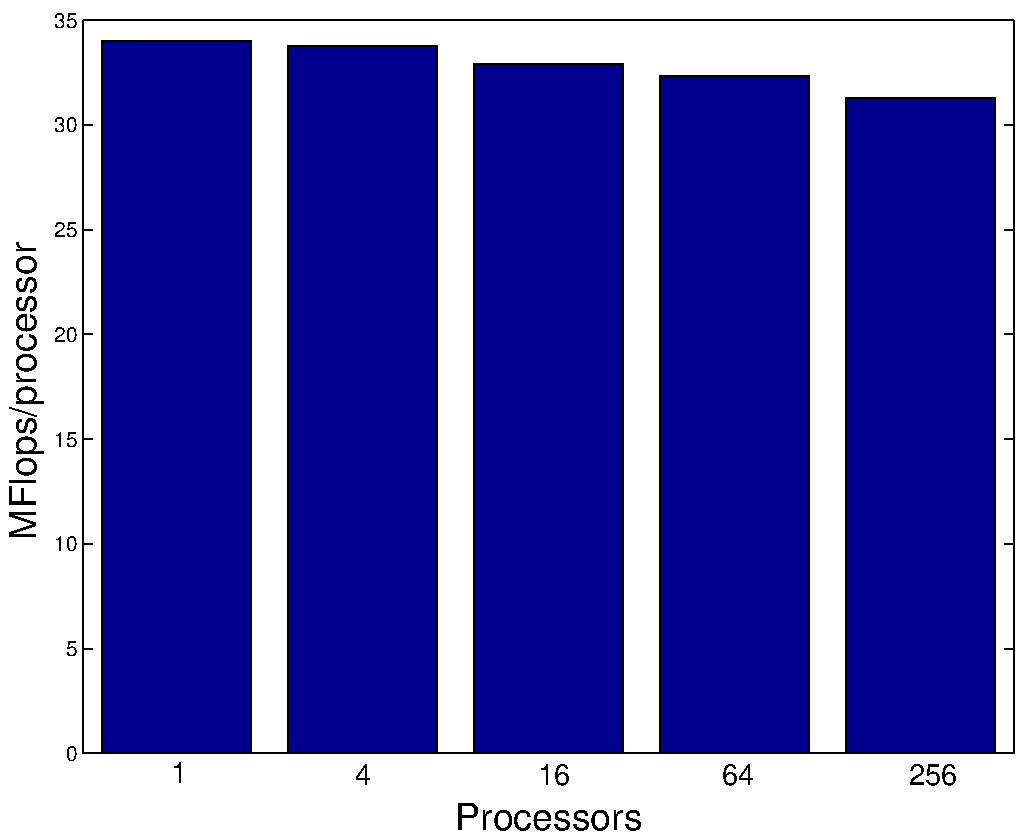
\includegraphics[height=1.8in]{../images/f3}
              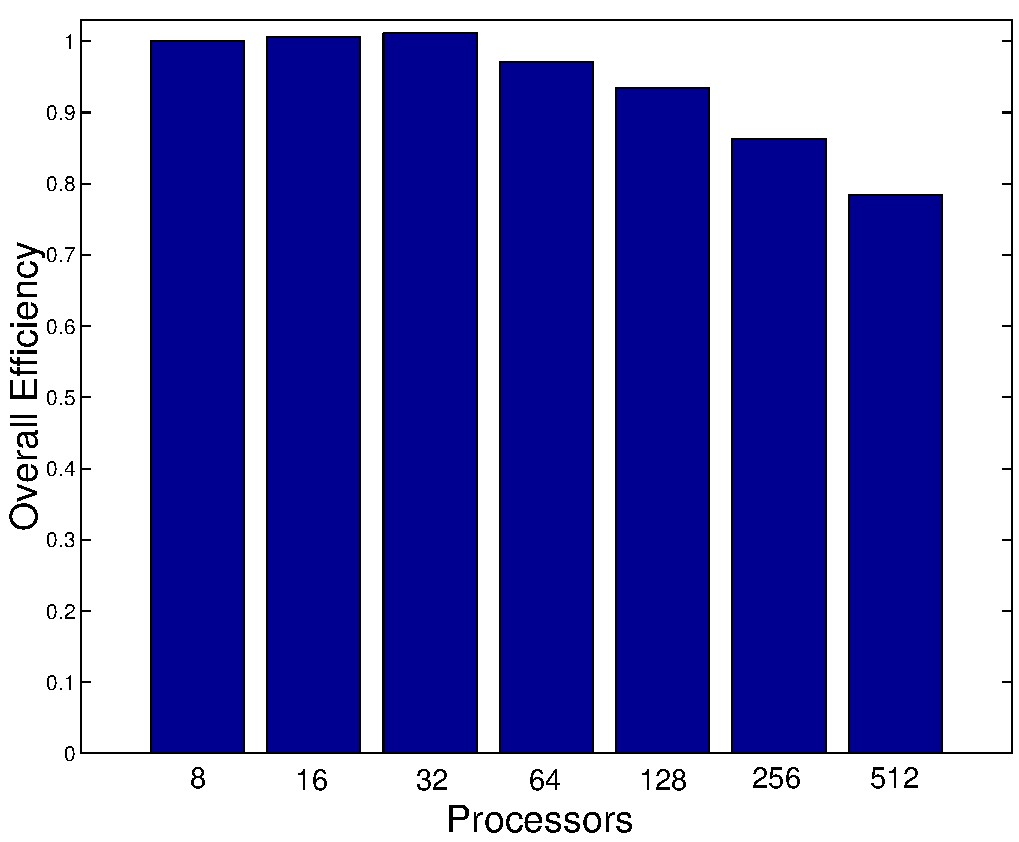
\includegraphics[height=1.8in]{../images/f4}}
\vfill

\end{slide}


\begin{slide}

\heading{TAO Algorithms (partial list)}

\begin{list}{\reddiamond}
{ \setlength{\itemsep}{0pt}}
\item
Unconstrained optimization 
\begin{list}{\reddash}{}
\item
Conjugate gradient algorithms PR, FR, PR+
\item
Levenberg-Marquardt method (alpha)
\end{list}
\item
Bound-constrained optimization
\begin{list}{\reddash}{}
\item
Limited-memory variable-metric algorithm
\item
Trust region Newton method
% \item
% Gradient projection/conjugate gradient algorithm
\end{list}
\item
Linearly constrained optimization
\begin{list}{\reddash}{}
\item
Interior-point quadratic programming  method (alpha)
\end{list}
\item
Nonlinearly constrained optimization
\begin{list}{\reddash}{}
\item
Work in progress
\end{list}
\end{list}

\vfill

\end{slide}

\begin{slide}

\heading{TAO Interface}

\begin{alltt}
\scriptsize \setlength{\baselineskip}{8pt}
  TAO_SOLVER tao;                   /* TAO_SOLVER solver context */
  Vec        x, g;                  /* solution and gradient vectors */
  int        n;                     /* number of variables */
  AppCtx     user;                  /* user-defined application context */
  TaoVecPetsc *xx,*gg;

  VecCreate(MPI_COMM_WORLD,n,&x);
  VecDuplicate(x,&g);

  TaoWrapPetscVec(x,&xx);
  TaoWrapPetscVec(g,&gg);

  TaoCreate(xx,''tao_lmvm'',0,MPI_COMM_WORLD,&tao);
  TaoSetFunctionGradient(tao,&ff,gg,FunctionGradient,(void *)&user);
  TaoSolve(tao);

  TaoDestroy(tao);
\end{alltt}

\vfill

\end{slide}

\begin{slide}

\heading{Function Evaluation}

\begin{alltt}
\scriptsize \setlength{\baselineskip}{8pt}
  typedef struct \{         /* Used in the minimum surface area problem */
    int         mx, my;            /* discretization in x, y directions */
    Vec         Bottom, Top, Left, Right;            /* boundary values */
  \} AppCtx;

  int FormFunction(TAO_SOLVER tao, TaoVec *xx, double* fcn,void *userCtx)\{
     AppCtx *user = (AppCtx *)userCtx;
     Vec X;

     TaoVecGetPetscVec(xx,&x);
     ...
     return 0;
  \}
\end{alltt}
The user sets this routine in the main program via
\begin{alltt}
\scriptsize \setlength{\baselineskip}{8pt}
    info = TaoSetFunction(tao,&ff,FormFunction,(void *)&user);
\end{alltt}

\vfill

\end{slide}

\begin{slide}

\heading{Gradient Evaluation}

\begin{alltt}
\scriptsize \setlength{\baselineskip}{8pt}
  int FormGradient(TAO_SOLVER tao, TaoVec *xx, TaoVec *gg,void *userCtx)\{
     AppCtx *user = (AppCtx *)userCtx;
     Vec X,G;

     TaoVecGetPetscVec(xx,&x);
     TaoVecGetPetscVec(gg,&g);
     ...
     return 0;
\}
\end{alltt}

The user sets this routine in the main program via
\begin{alltt}
\scriptsize \setlength{\baselineskip}{8pt}
    info = TaoSetGradient(tao,gg,FormGradient,(void *)&user);
\end{alltt}
Alternatively, the user can supply the function and gradient evaluation
in a single routine.

\medskip

A Hessian evaluation routine can be supplied in a similar manner.

\vfill

\end{slide}

\begin{slide}

\heading{Convergence}

\vfill

\end{slide}

\begin{slide}

\heading{TAO Basic Facilities}

\begin{list}{\reddiamond}{}
\item
TaoSetInitialVector
\item
TaoSetBounds
\item
TaoGetLinearSolver
\item 
TaoGetIterationData
\item
TaoView
\end{list}

\vfill

\end{slide}

\begin{slide}

\heading{Parallel Functionality}

The TAO interface is the same in a parallel environment, but the user
must provide vectors with a parallel structure.
\begin{alltt}
\scriptsize \setlength{\baselineskip}{8pt}
  VecCreateMPI(MPI_COMM_WORLD,n,PETSC_DECIDE,&x);
  VecDuplicate(x,&g);

  TaoWrapPetscVec(x,&xx);
  TaoWrapPetscVec(g,&gg);
  info = TaoCreate(xx,''tao_lmvm'',0,MPI_COMM_WORLD,&tao);
  info = TaoSetFunctionGradient(tao,ff,gg,FunctionGradient,(void *)&user);
  info = TaoSolve(tao);

  info = TaoDestroy(tao);
\end{alltt}
The user still provides the routines that evaluate the function and
gradient.  These routines do not have to be performed in parallel,
but parallel evaluations usually improve performance.
\end{slide}


\begin{slide}

\heading{Parallel Function Evaluation}

\begin{alltt}
\scriptsize \setlength{\baselineskip}{8pt}
   typedef struct \{                    /* For Minimum Surface Area Problem */
     int         mx, my;              /* discretization in x, y directions */
     Vec         Bottom, Top, Left, Right;              /* boundary values */
     DA          da;                   /* distributed array data structure */
   \} AppCtx;

   int FormFunction(TAO_SOLVER tao, TaoVec *xx, double* fcn,void *userCtx)\{
      AppCtx *user = (AppCtx *)userCtx;
      Vec x;
      double f=0;
      TaoVecGetPetscVec(xx,&x);
      for (i=xs; i<xe; i++)\{
        for (j=ys; j<ye; j++)\{
           f += ...
        \}
      \}
      info = MPI_Allreduce(&f,fcn,1,MPI_DOUBLE,MPI_SUM,MPI_COMM_WORLD);
      return 0;
   \}
\end{alltt}

\vfill

\end{slide}

\begin{slide}

\heading{TAO}

\begin{center}
\href{http://www.mcs.anl.gov/tao}{www.mcs.anl.gov/tao} \\
Version 1.2 (June 2001)
\end{center}


\begin{list}{\reddiamond}{}
\item
Source Code
\item
\href{http://www.mcs.anl.gov/tao/docs}
{Documentation}
\item
Installation instructions
\item
\href{http://www-unix.mcs.anl.gov/tao/src/bound/examples/exercises/main.htm}%
{Example problems}
\item
Performance results
\item
Supported architectures
\end{list}

\vfill

\end{slide}

\end{document}


\begin{slide}

\heading{}

\begin{list}{\reddiamond}{}
\item

\end{list}

\vfill

\end{slide}
